\documentclass[beamer]{standalone}
\usepackage{circuitikz}
\begin{document}

\title[Electronics 1]{Diodes}

\begin{frame} 
  \titlepage
\end{frame}


\section{Midterm exam notes}
\begin{frame}
 \frametitle{Midterm exam: Week of March 2nd}
  Where: In the lab

  When: During the first hour of the lab

  Material (\alert{textbook only} allowed during midterm): 
  \begin{itemize}
    \item Everything, including today (Chapter 1--4)
    \item Resistors, capacitors, inductors, and transformers.
    \item Kirchhoff's laws
    \item Complex impedance.
    \item Th\'{e}venin's theorem
      \begin{itemize}
        \item Source impedance and voltage
      \end{itemize}
    \item Voltage divider in various forms
    \item Filters (only sections included in reading)
    \item Diodes (focus on 4.5--6, no details on band gap etc.)
  \end{itemize}

  \alert{Lab will follow the midterm.}

  You can skip the design exercise preparation prior to the lab. However, at the time of log book submission it must be fully done. Treat it as home work.
\end{frame}
  
\section{Band Structure}
\begin{frame}[t]
 \frametitle{Band gap structure in periodic lattice}
 \begin{block}{Fermi energy $E_F$ in band gap}
  \begin{center}
   \pgfimage[width=0.7\textwidth]{pics/bandgap}
  \end{center}
 \end{block}
\end{frame}

\begin{frame}[t]
 \frametitle{Band gap structure in periodic lattice}
 \begin{columns}[t]
  \begin{column}{0.47\textwidth}
   \begin{block}{n-type doping}
    \pgfimage[width=\textwidth]{pics/bands_n}
   \end{block}
  \end{column}
  \begin{column}{0.49\textwidth}
   \begin{block}{p-type doping}
    \pgfimage[width=\textwidth]{pics/bands_p}
   \end{block}
  \end{column}
 \end{columns}
\end{frame}

\begin{frame}
\frametitle{Semiconductors and doping}
 \begin{columns}[t]
  \begin{column}{.3\textwidth}
    Pure semiconductor
    \begin{figure}
      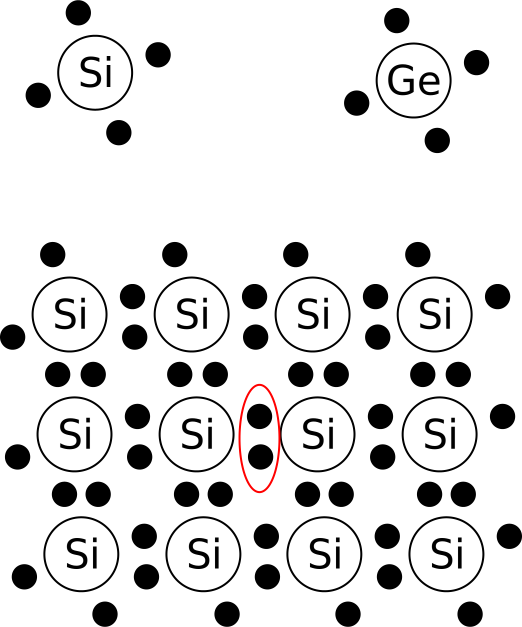
\includegraphics[width=0.80\textwidth]{./pics/semiconductor}
    \end{figure}
  \end{column}
  \begin{column}<2->{.3\textwidth}
    P-doped
    \begin{figure}
      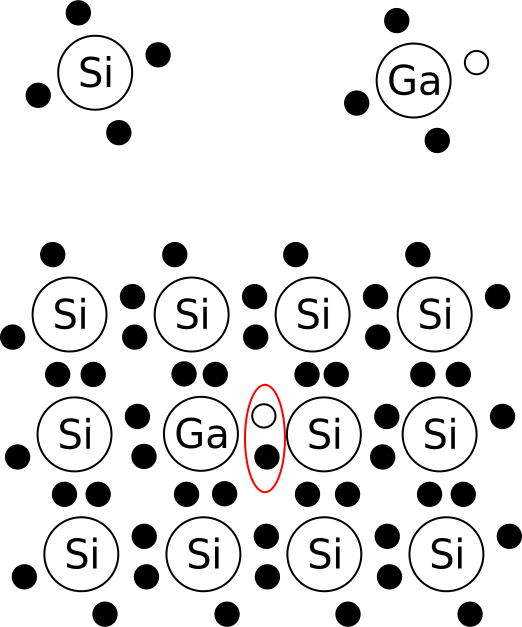
\includegraphics[width=0.80\textwidth]{./pics/pdopped}
    \end{figure}
  \end{column}
  \begin{column}<3->{.3\textwidth}
    N-doped
    \begin{figure}
      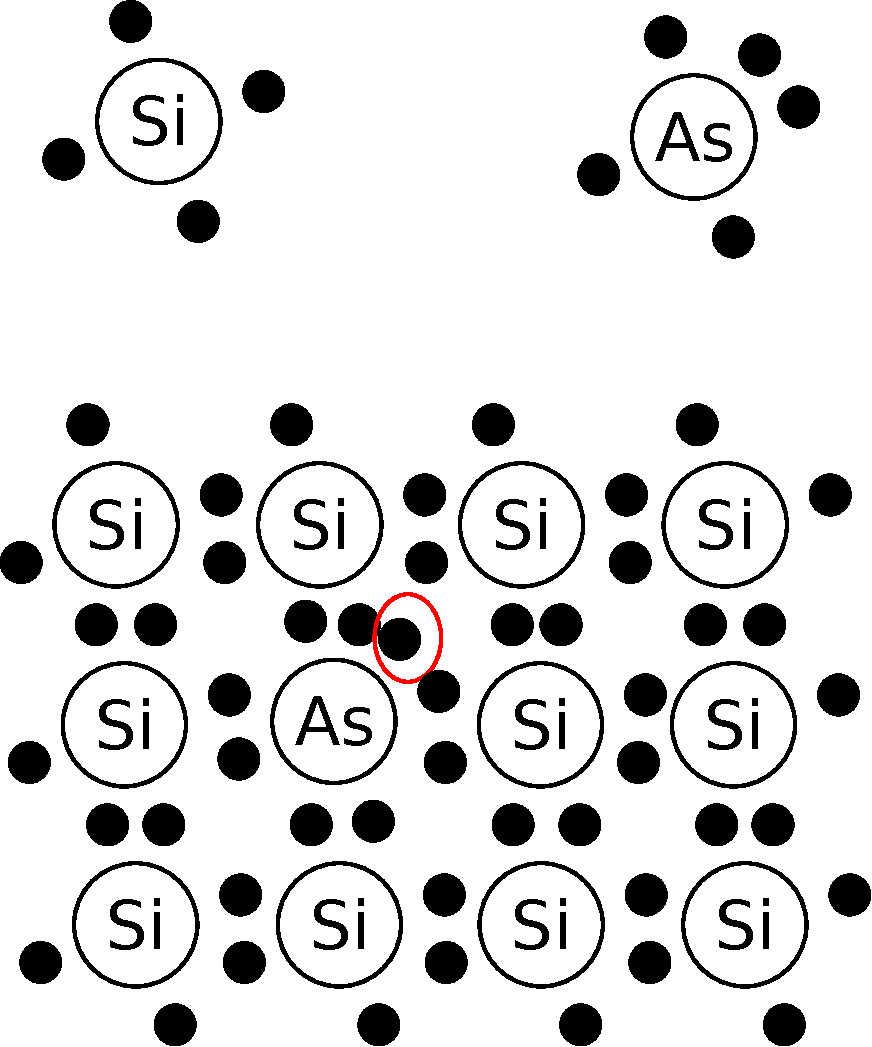
\includegraphics[width=0.80\textwidth]{./pics/ndopped}
    \end{figure}
  \end{column}
 \end{columns}
\end{frame}

\begin{frame}
 \frametitle{pn-junction}
 \begin{block}{Diffusion at pn interface}
  \begin{center}
   \pgfimage[width=0.5\textwidth]{pics/pn_junction}
  \end{center}
  Potential difference builds up, n-type at higher potential due to positive holes.
 \end{block}
\end{frame}


\frame
{ \frametitle{pn-junction} %{{
\begin{columns}[t]
  \begin{column}{.3\textwidth}
    No bias
    \begin{figure}
      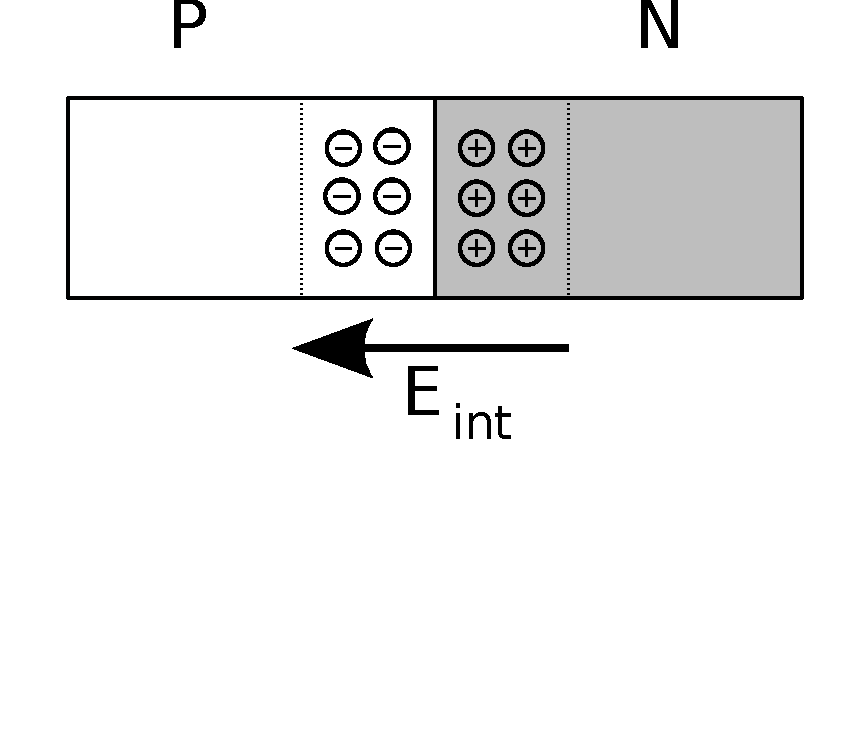
\includegraphics[width=0.80\textwidth]{./pics/pnjunction_nobias}
    \end{figure}
  \end{column}
  \begin{column}<2->{.3\textwidth}
    Reverse bias
    \begin{figure}
      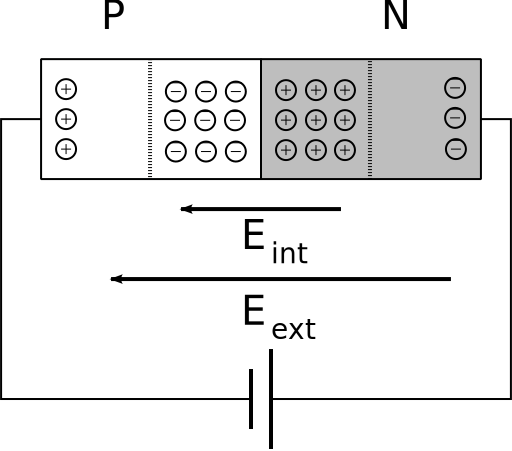
\includegraphics[width=0.80\textwidth]{./pics/pnjunction_reverse_bias}
    \end{figure}
  \end{column}
  \begin{column}<3->{.3\textwidth}
    Forward bias
    \begin{figure}
      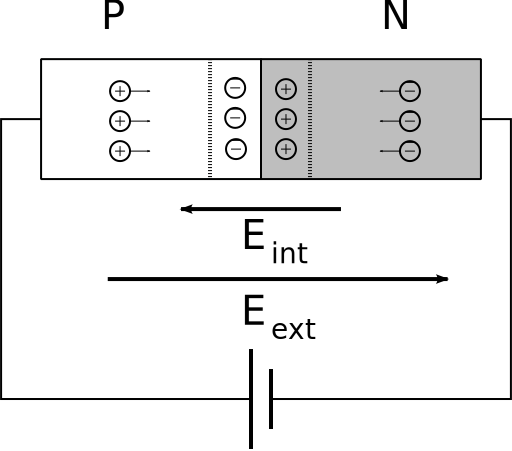
\includegraphics[width=0.80\textwidth]{./pics/pnjunction_forward_bias}
    \end{figure}
  \end{column}
\end{columns}
  }

  
\section{Diodes}

\frame
{ \frametitle{Ideal diode}
\begin{figure}
  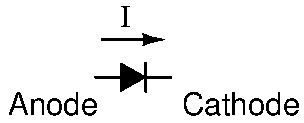
\includegraphics[width=0.30\textwidth]{./schematics/diode}
\end{figure}
\begin{figure}
  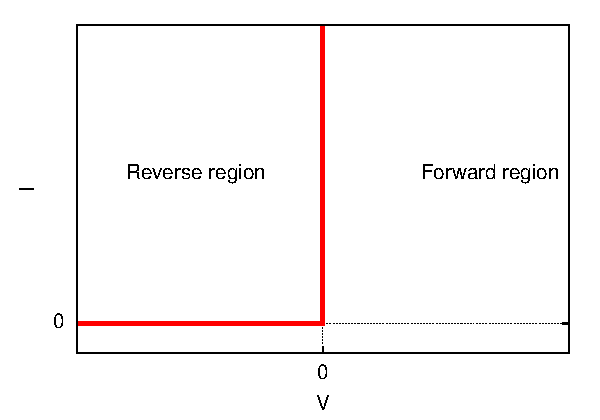
\includegraphics[angle=0,width=0.70\textwidth]{./plots/ideal_diode}
\end{figure}
}

\begin{frame}
\frametitle{Real diode}
\vskip -.2in
\begin{figure}
  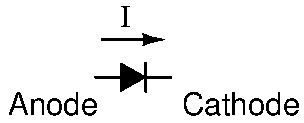
\includegraphics[width=0.30\textwidth]{./schematics/diode}
\end{figure}

\vskip -.2in
\begin{columns}[t]
  \begin{column}{.35\textwidth}
    \[
    I(V)=I_S\left( e^{{V}/(m V_{T})}-1 \right) 
    \]
    Typical parameters
    \begin{itemize}
      \item saturation current $I_S=1$~nA
      \item thermal voltage $V_T=\frac{kT}{q}=25.85$~mV at 300~K
      \item emission coefficient $m=1..2$
    \end{itemize}
    
  \end{column}
  \begin{column}{.65\textwidth}
    \begin{figure}
      \includegraphics<1>[angle=0,width=1.00\textwidth]{./plots/realistic_diode}
      \includegraphics<2>[angle=0,width=1.00\textwidth]{./plots/diode_combined}
    \end{figure}
  \end{column}
\end{columns}
\end{frame}

\frame
{ \frametitle{Simplified diode}
\begin{figure}
  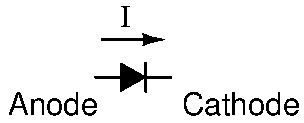
\includegraphics[width=0.30\textwidth]{./schematics/diode}
\end{figure}
\vskip -.5in
\begin{columns}[c]
  \begin{column}{.55\textwidth}
    $V_{pn}$ diode pn junction opening voltage
    \begin{itemize}
      \item $V_{pn}=0.6$~V for Si
      \item $V_{pn}=0.3$~V for Ge
    \end{itemize}
  \end{column}
  \begin{column}{.45\textwidth}
    \begin{figure}
      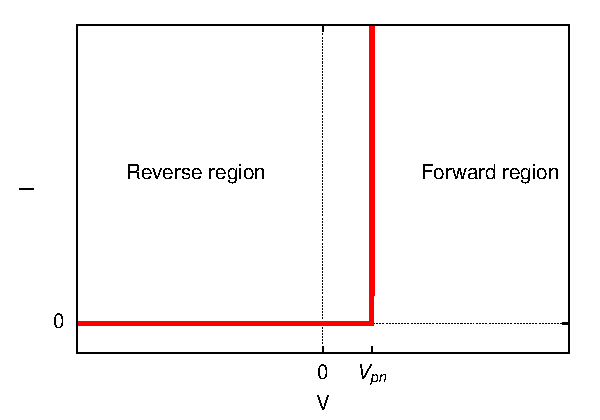
\includegraphics[angle=0,width=1.00\textwidth]{./plots/simplified_diode}
    \end{figure}
  \end{column}
\end{columns}
\vskip -.2in
\begin{columns}[c]
  \begin{column}{.35\textwidth}
    A bit more realistic diode ($R_r \gg R_f$)
  \end{column}
  \begin{column}{.35\textwidth}
    \begin{figure}
      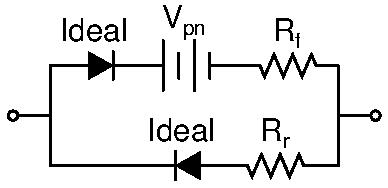
\includegraphics[width=1.00\textwidth]{./schematics/real_diode_model}
    \end{figure}
  \end{column}
\end{columns}
}

\section{Diodes applications}
\frame
{ \frametitle{Diodes applications}
\begin{itemize}
  \item 
    Circuit Protection
  \item 
    Rectification
    \begin{itemize}
      \item Current gate
      \item Half-wave rectifier
      \item Full-wave rectifier
      \item Power Supplies
    \end{itemize}
  \item 
    Frequency manipulation
    \begin{itemize}
      \item Frequency multiplier
      \item Mixers
    \end{itemize}
  \item 
    and more \ldots
    \begin{itemize}
      \item Voltage clamps
      \item Light emitting diodes (LED)
      \item Photo-diodes
    \end{itemize}
\end{itemize}
}
  

\section{Half-wave rectifier}
\frame
{ \frametitle{Half-wave rectifier, current gate}
  \begin{figure}
    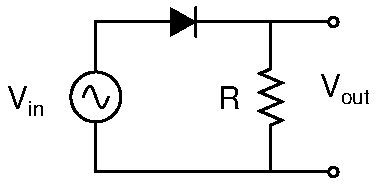
\includegraphics[width=0.30\textwidth]{./schematics/half_wave_rectifier}
  \end{figure}
  \vskip -.5in
    \begin{figure}
      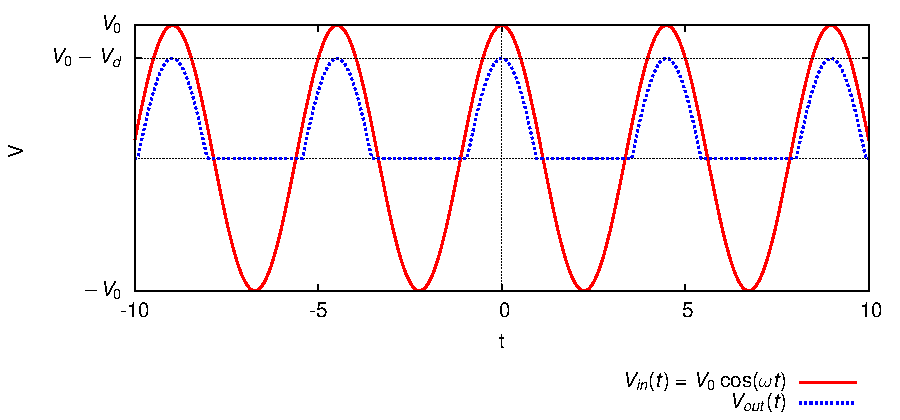
\includegraphics[angle=0,width=1.00\textwidth]{./plots/half_wave_rectifier}
    \end{figure}
  }

  
\section{Full-wave rectifier}
\begin{frame}
 \frametitle{Full-wave rectifier: $V_{in} \gg V_d \to V_{out} \approx | V_{in}|$}
  \begin{columns}[c]
    \begin{column}{.50\textwidth}
  \begin{figure}
    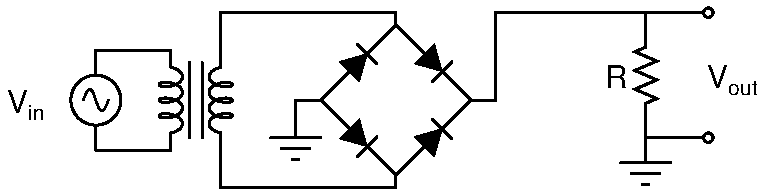
\includegraphics[width=0.90\columnwidth]{./schematics/full_wave_rectifier}
  \end{figure}
    \end{column}
    \begin{column}{.50\textwidth}
      Why $\max(V_{out}) = V_0 - \alert{2 V_d} $ ? \\
      Why transformer?
    \end{column}
  \end{columns}
  %\vskip -.5in
    \begin{figure}
      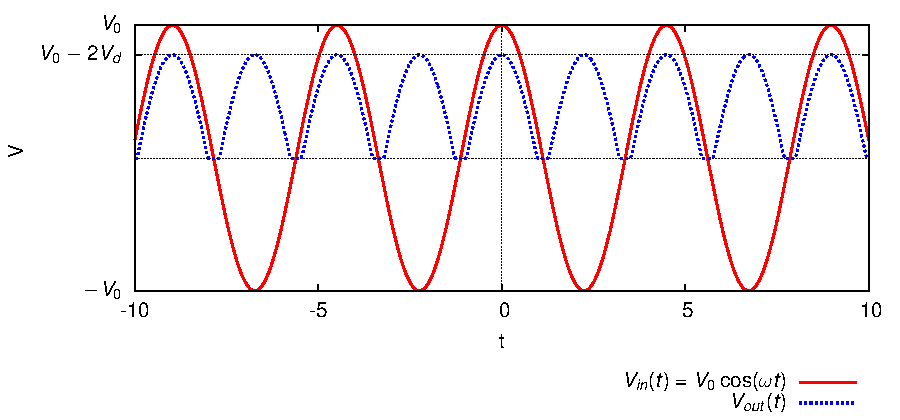
\includegraphics[angle=0,width=1.00\columnwidth]{./plots/full_wave_rectifier}
    \end{figure}
\end{frame}
  
\begin{frame}
 \frametitle{Full-wave rectifier filtered - power supply}
  \begin{columns}[t]
    \begin{column}{.55\textwidth}
  \vskip -.3in
      \begin{figure}
        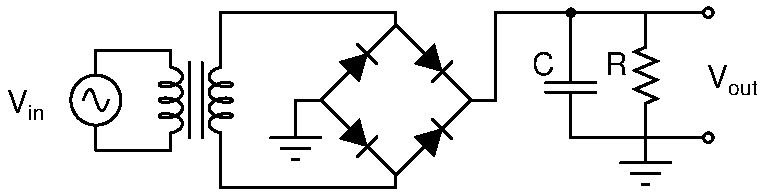
\includegraphics[width=1.00\textwidth]{./schematics/full_wave_rectifier_filtered}
      \end{figure}
  \vskip -.3in
      \begin{figure}
        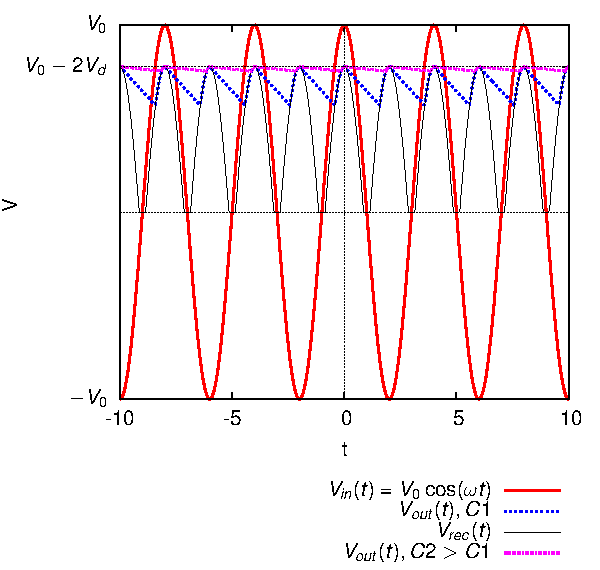
\includegraphics[angle=0,width=1.00\textwidth]{./plots/full_wave_rectifier_filtered}
      \end{figure}
    \end{column}
    \begin{column}{.45\textwidth}
      Ripples size
      \begin{eqnarray*}
        v(t) & = & \frac{q(t)}{C} = \frac{Q_{max}- \int_0^t i dt}{C} \\
             & = & V_{max} - \int_0^t \frac{i}{C} dt\\
          \Delta v & = &  V_{max} - v(t) = \int_0^t \frac{i}{C} dt\\
        I &\le& I_{max} = \frac{V_{max}} {R} \\
        t &\le& T = \frac{1}{2 f_{in}} \\
      \end{eqnarray*}
      \vskip -.3in
      \begin{block}{\alert{$T \ll RC$} }
      \vskip -.1in
        \begin{eqnarray*}
          \Delta V &\le&  \frac{V_{max}}{2 R C f_{in}} 
        \end{eqnarray*}
      \end{block}
    \end{column}
  \end{columns}
\end{frame}
  
\section{Frequencies doubling and summing}
\begin{frame}
 \frametitle{Full-wave rectifier as Frequency doubler}
  \begin{figure}
    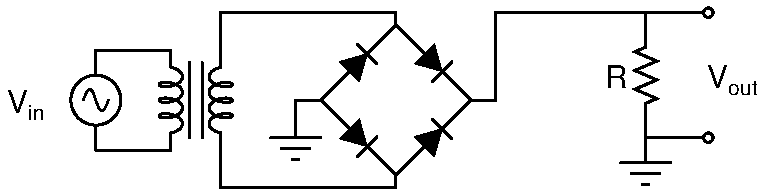
\includegraphics[width=0.60\textwidth]{./schematics/full_wave_rectifier}
  \end{figure}
  \vskip -.6in
  \begin{columns}[c]
    \begin{column}<1->{.45\textwidth}
    \begin{figure}
      \includegraphics<1>[angle=0,width=1.00\textwidth]{./plots/full_wave_rectifier}
      \includegraphics<2->[angle=0,width=1.00\textwidth]{./plots/full_wave_rectifier_as_doubler}
    \end{figure}
    \end{column}
    \begin{column}<3->{.1\textwidth}
      FFT \\
      {\Huge
      $\Rightarrow$
      }
    \end{column}
    \begin{column}<4->{.45\textwidth}
    \begin{figure}
      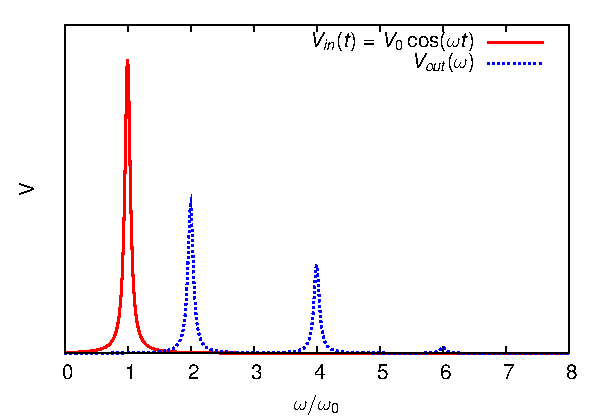
\includegraphics[angle=0,width=1.00\textwidth]{./plots/freq_doubler}
    \end{figure}
    \end{column}
  \end{columns}
  \vskip -.5in
\end{frame}
  

\begin{frame}
 \frametitle{ Full-wave rectifier as Frequency adder}
  \begin{figure}
    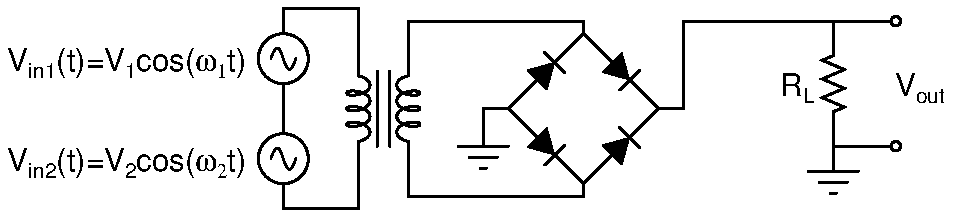
\includegraphics[width=0.60\textwidth]{./schematics/full_wave_rectifier_as_adder}
  \end{figure}
      \begin{eqnarray*}
        v_{out}(t) 
        & = & |v_{in}(t)| = \sqrt{v_{in}^2(t)} = \sqrt{ \left( V_1 \cos(\omega_1 t) + V_2 \cos(\omega_2 t) \right)^2  } \\
        &=& \sqrt{  
        V_1^2 \cos^2(\omega_1 t) 
        + 2 V_1 V_2 \cos(\omega_1 t) \cos(\omega_2 t) 
        + V_2^2 \cos^2(\omega_2 t) 
        }
      \end{eqnarray*}
      Assuming $V_1 \gg V_2$
      \begin{eqnarray*}
        v_{out}(t) 
        &\approx&  
        \sqrt{ V_1^2 \cos^2(\omega_1 t) + 2 V_1 V_2
        \cos(\omega_1 t) \cos(\omega_2 t) 
        +\rlap{------------------}{ V_2^2 \cos^2(\omega_2 t) }
        } \\
        &\approx&  
        V_1 \left( \cos(\omega_1 t) + \frac{V_2}{V_1} \cos(\omega_1 t)
        \cos(\omega_2 t) \right) \\
        &\approx&  
        V_1 \left( 
          \cos(\omega_1 t) 
          + \frac{V_2}{V_1} 
            \frac{
              \cos( (\omega_1 +\omega_2) t) + \cos( (\omega_1 -\omega_2) t)  
              }{2}
        \right)
      \end{eqnarray*}
\end{frame}
  
\end{document}
